\textbf{Verificación subsistema 6}
Para verificar la estructura fue necesario montar los diferentes componentes mecánicos que integran el proyecto, de tal forma que no solo se verificó la rigidez y estabilidad de la estructura, sino también que los distintos componentes pudieran situarse de manera adecuada a la estructura.

 \begin{figure}[h]
            \centering
            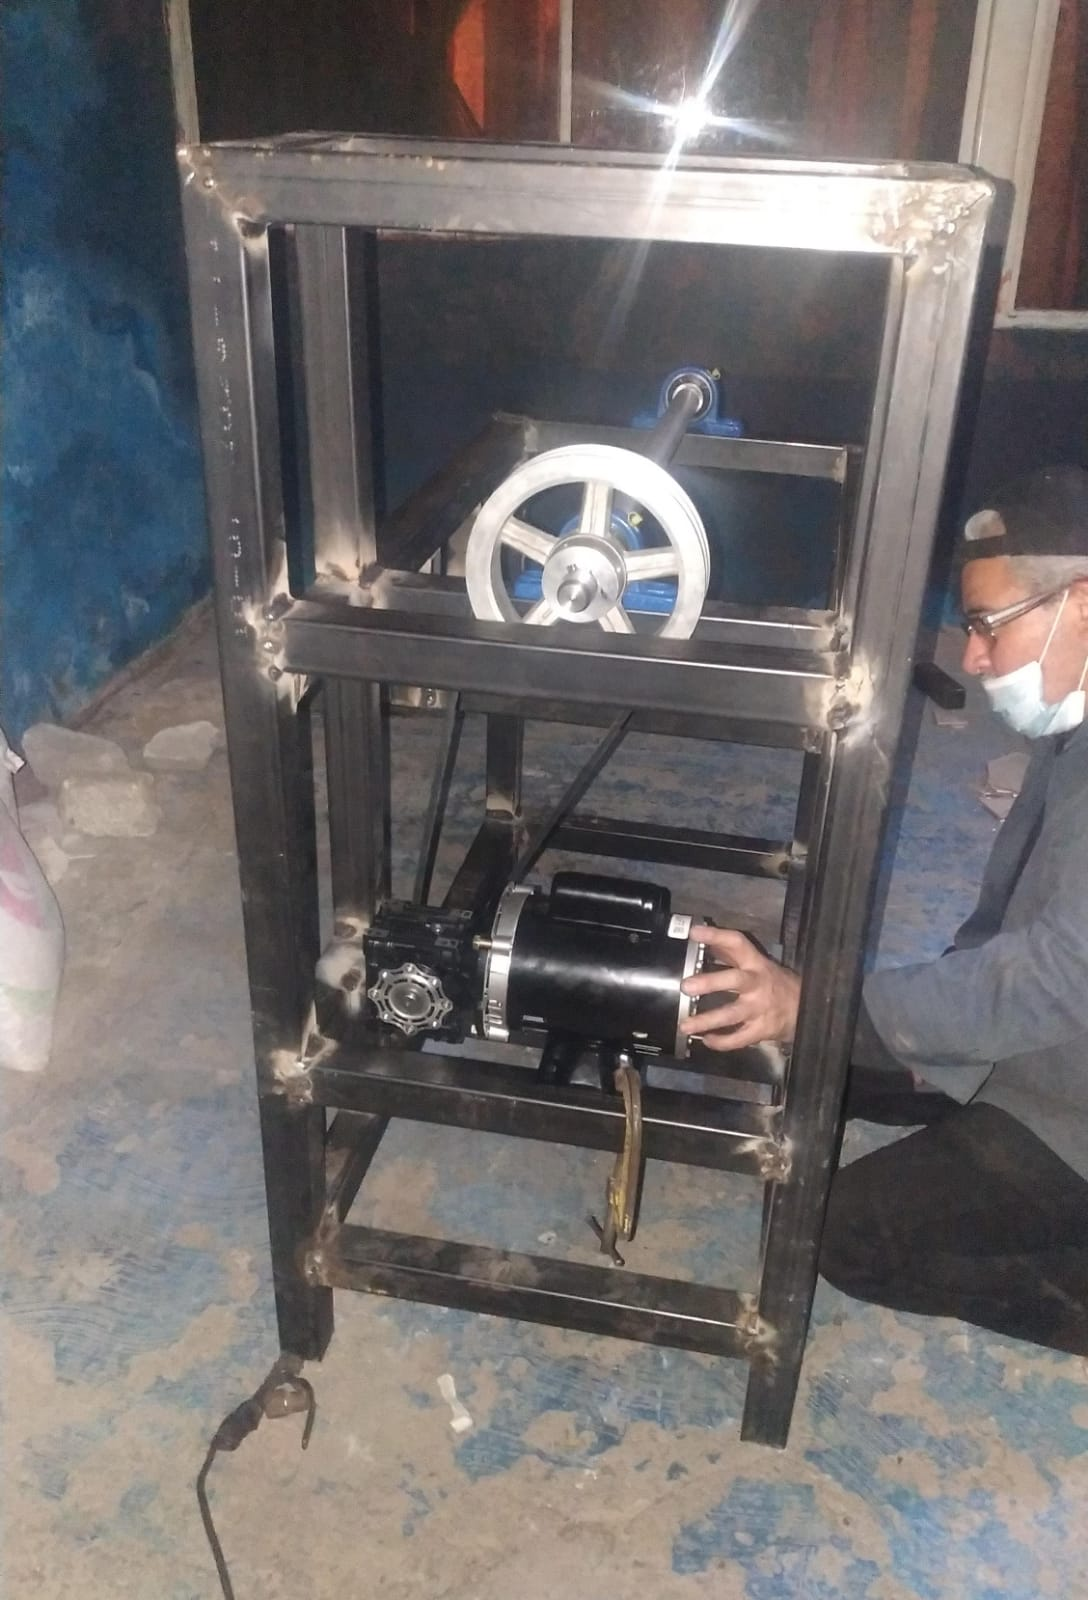
\includegraphics[scale=0.135]{images/Pruebas_S6/montar_componentes.jpeg}
            \caption{Montaje de componentes en estructura}
            \label{fg:estructura elaborada}
 \end{figure}

A diferencia del modelo 3D que se tenía en un inicio para la estructura, fue necesario agregar soportes que permitieran colocar el motor para el sistema de trituración, teniendo como resultado una estructura apta para integrar todos los componentes y mecanismos necesarios para el correcto funcionamiento del sistema.

Durante la realización de la estructura resaltó la necesidad de disminuir el espacio donde se colocaría el contenedor, ya que existía un espacio de aproximadamente media pulgada entre las paredes laterales del contenedor y los lados de la estructura, también se redujo a lo largo una pulgada, para que el contenedor no pudiera desplazarse de atrás hacia adelante.

Finalmente fue necesario colocar soportes que permitieran fijar el triturador y el motor de aireación, ya que en un inicio se consideró colocar una placa de acero, sin embargo se opto por soldar PTR debido a que resultaba más fácil y barato que adquirir una placa de acero con el suficiente espesor para evitar deformaciones.
\newpage